\documentclass{article}
\usepackage{graphicx} % Required for inserting images
\usepackage{amsmath}  % Required for align environment
\usepackage{tikz}
\usetikzlibrary{arrows,shapes,positioning}
\usepackage[margin=1in]{geometry}


\title{ELCT 432 Assignment \#3}
\author{Jacob C. Vaught}
\date{September 13-16th 2023}

\begin{document}
\maketitle

\newpage
\section*{Problem \#1}
Consider DSB-SC AM \( u(t) = m(t)c(t) \) where the message signal \( m(t) = \cos(40t) + 2\sin \left(50t + \frac{\pi}{4}\right) \) modulates the carrier signal \( c(t) = A\cos(2\pi f_c t) \). Assume that \( f_c = 4 \, \text{kHz} \).

\subsection*{Tasks}
\begin{enumerate}
    \item Find the frequency-domain representations of the modulated signal.
    \item Plot the spectrum (i.e., Fourier Transform) of the modulated signal (i.e., draw both \( |U(f)| \) and \( \angle U(f) \)).
    \item Calculate the power content of the modulated signal.
\end{enumerate}

\subsection*{Solutions}
\subsection*{a) Frequency-Domain Representations}

To find the frequency-domain representation of the modulated signal, we first need to understand the frequency-domain representations of the individual message and carrier signals.

\begin{itemize}
    \item Step 1: Fourier Transform of the message signal \( m(t) \)
    \[
    M(f) = \mathcal{F}\{\cos(40t)\} + 2\mathcal{F}\{\sin(50t + \frac{\pi}{4})\}
    \]
    Breaking this down, the Fourier Transform of \( \cos(40t) \) is:
    \[
    \frac{1}{2}[\delta(f - \frac{40}{2\pi}) + \delta(f + \frac{40}{2\pi})]
    \]
    And for \( \sin(50t + \frac{\pi}{4}) \), it is:
    \[
    -\frac{j}{2} \left( e^{j\frac{\pi}{4}}\delta(f - \frac{50}{2\pi}) - e^{-j\frac{\pi}{4}}\delta(f + \frac{50}{2\pi}) \right)
    \]
    Combining these, we get:
    \[
    M(f) = \frac{1}{2}[\delta(f - \frac{40}{2\pi}) + \delta(f + \frac{40}{2\pi})] - j\frac{1}{2}[\delta(f - \frac{50}{2\pi}) - \delta(f + \frac{50}{2\pi})]
    \]
    
    \item Step 2: Fourier Transform of the carrier signal \( c(t) \)
    \[
    C(f) = \mathcal{F}\{A\cos(2\pi f_c t)\}
    \]
    Simplifying, we get:
    \[
    C(f) = \frac{A}{2}[\delta(f - 4000) + \delta(f + 4000)]
    \]
    
    \item Step 3: Frequency-Domain Representation of the modulated signal \( u(t) \)
    Now we find \( U(f) \), which is essentially \( M(f) \times C(f) \).
\begin{align*}
U(f) = \frac{A}{4} \Big[ &\delta\left(f - 4000 - \frac{40}{2\pi}\right) + \delta\left(f + 4000 + \frac{40}{2\pi}\right) + \delta\left(f - 4000 + \frac{40}{2\pi}\right) + \delta\left(f + 4000 - \frac{40}{2\pi}\right) \\
& - j\delta\left(f - 4000 - \frac{50}{2\pi}\right) + j\delta\left(f + 4000 + \frac{50}{2\pi}\right) + j\delta\left(f - 4000 + \frac{50}{2\pi}\right) - j\delta\left(f + 4000 - \frac{50}{2\pi}\right) \Big]
\end{align*}


\end{itemize}
\newpage
\subsection*{b) Plotting the Spectrum}

The spectrum of \( U(f) \) is best understood visually. To plot the spectrum, we have used MATLAB to generate Figure~\ref{fig:spectrum_plot}.

\begin{figure}[h]
    \centering
    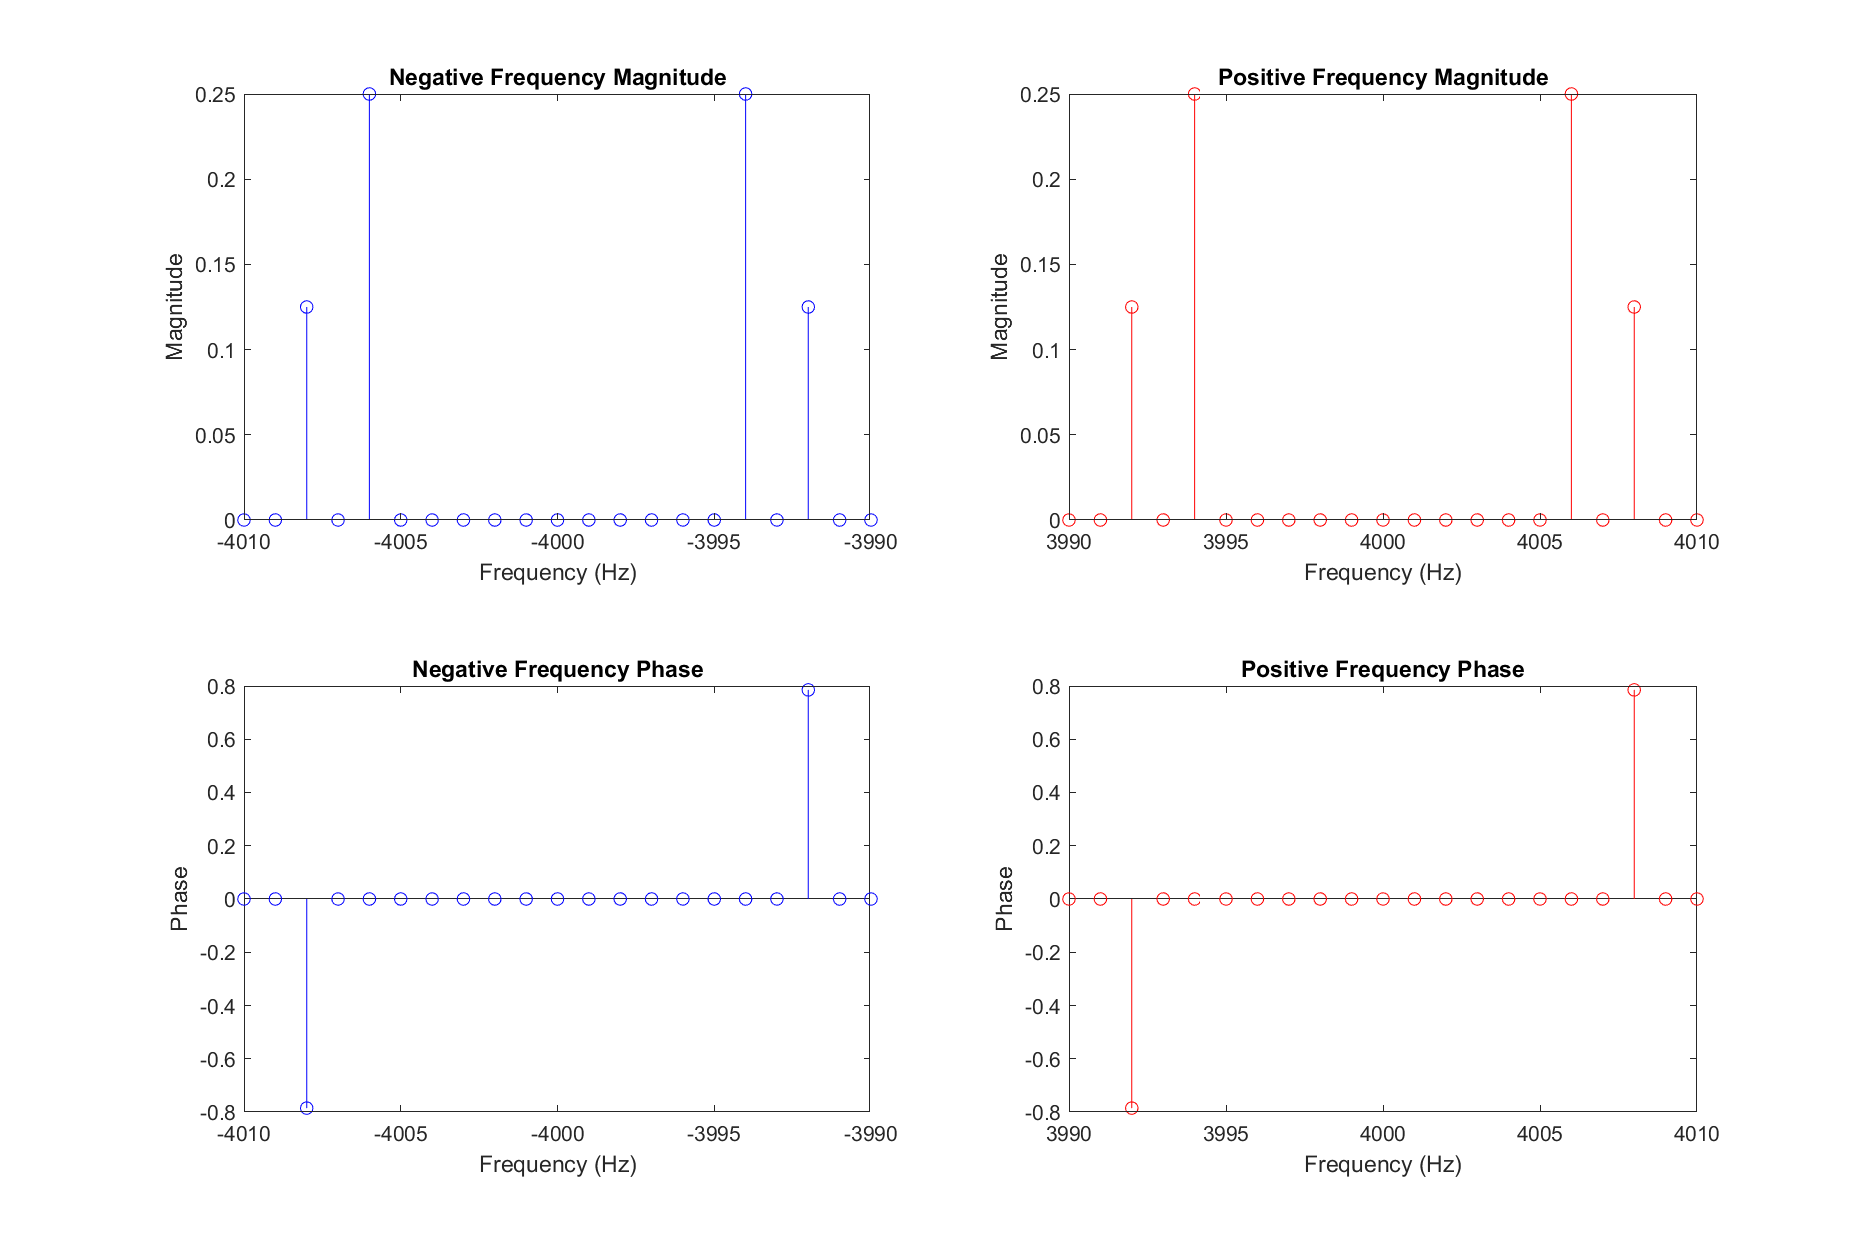
\includegraphics[width=1\textwidth]{spectrum_plot.png}
    \caption{Spectrum of \( U(f) \)}
    \label{fig:spectrum_plot}
\end{figure}

\subsection*{c) Calculating the Power Content}

To find the power content of the modulated signal \( u(t) \), we integrate \( |U(f)|^2 \) over all frequencies.Note that anytime there is a shift by 40 or 50, It should say $\frac{40 or 50}{2 pi}$

\[
P = \frac{1}{2\pi} \int_{-\infty}^{+\infty} |U(f)|^2 \, df
\]
Here, \( U(f) \) is:
\begin{align*}
U(f) &= \frac{A}{4} \Bigg[ \delta(f - 4040) + \delta(f + 4040) + \delta(f - 3960) + \delta(f + 3960) \\
& \quad - j\delta(f - 4050) + j\delta(f + 4050) + j\delta(f - 3950) - j\delta(f + 3950) \Bigg]
\end{align*}

Squaring the magnitude, \( |U(f)|^2 \), yields:
\begin{align*}
|U(f)|^2 &= \left(\frac{A}{4}\right)^2 \Bigg[ \delta^2(f - 4040) + \delta^2(f + 4040) \\
& \quad + \delta^2(f - 3960) + \delta^2(f + 3960) + \delta^2(f - 4050) \\
& \quad + \delta^2(f + 4050) + \delta^2(f - 3950) + \delta^2(f + 3950) \Bigg]
\end{align*}

At this point, it's crucial to understand the nature of the Dirac delta function \(\delta(f)\). In the context of integration, the delta function acts like an "infinitely tall and infinitely narrow" spike at the origin, with the area under the curve being 1. This means that when we integrate \( |U(f)|^2 \) over all frequencies, the integral at those specific frequencies (i.e., \(f = \pm 4040, \pm 3960, \pm 4050, \pm 3950\)) will each contribute a value of 1 to the overall sum.

\[
P = \frac{1}{2\pi} \left(\frac{A}{4}\right)^2 \times 8
\]
This simplifies to:
\[
P = \frac{A^2}{8}
\]
Chegg says it should be 16, but my calculations said 8.
\[
P = \frac{A^2}{16}
\]


\newpage
\section*{Problem \#2}
Prove that \(\text{sinc}(t) * \text{sinc}(t) = \text{sinc}(t)\), where \( * \) denotes the convolution operation. Hint: Use the Convolution Theorem. 

\subsection*{Solution}
\subsection*{Convolution Theorem and Fourier Transform}
The Convolution Theorem states that the Fourier Transform of a convolution of two signals is equal to the product of their Fourier Transforms. Mathematically, if \( f(t) * g(t) = h(t) \), then \( \mathcal{F}\{ h(t) \} = \mathcal{F}\{ f(t) \} \times \mathcal{F}\{ g(t) \} \).

\subsection*{Fourier Transform of sinc(t)}
The Fourier Transform of \( \text{sinc}(t) \), which is defined as \( \frac{\sin(\pi t)}{\pi t} \), is a rectangular function \( \text{rect}(f) \), often denoted as \( \Pi(f) \), where \( \Pi(f) = 1 \) for \( |f| < \frac{1}{2} \) and \( \Pi(f) = 0 \) elsewhere.

\subsection*{Applying the Convolution Theorem}
We are interested in proving \( \text{sinc}(t) * \text{sinc}(t) = \text{sinc}(t) \).
\newline \newline
Taking the Fourier Transform of \( \text{sinc}(t) * \text{sinc}(t) \) and applying the Convolution Theorem, we get:
\[
\mathcal{F}\{ \text{sinc}(t) * \text{sinc}(t) \} = \Pi(f) \times \Pi(f) = \Pi(f)
\]
Here \( \Pi(f) \times \Pi(f) = \Pi(f) \) because the multiplication of two identical rectangular functions remains the same rectangular function.

\subsection*{Inverse Fourier Transform}
Since \( \mathcal{F}\{ \text{sinc}(t) * \text{sinc}(t) \} = \Pi(f) \), taking the inverse Fourier Transform yields:
\[
\text{sinc}(t) * \text{sinc}(t) = \text{sinc}(t)
\]
This concludes the proof.

\newpage
\section*{Problem \#3}
Consider DSB-SC AM. Assume that the carrier is \( c(t) = A \cos(2\pi f_c t) \). Assume that the message signal is \( m(t) = \text{sinc}(t)\text{sinc}(t) + \text{sinc}(t) \star \text{sinc}(t) \), where \( \star \) denotes the convolution operation. 
\begin{enumerate}
    \item What is the bandwidth of the modulated signal (i.e., passband signal)?
    \item Find the frequency domain expression of the DSB-AM signal.
\end{enumerate}

\subsection*{Solutions}

\subsection*{a) Bandwidth of the Modulated Signal}
To find the bandwidth of the modulated signal, we first need to determine the bandwidth of \( m(t) \). Recall that the Fourier Transform of \( \text{sinc}(t) \) is \( \text{rect}(f) \), a rectangular pulse extending from \( -\frac{1}{2} \) to \( \frac{1}{2} \). Thus, the bandwidth of \( \text{sinc}(t) \) is 1. The convolution and product of \( \text{sinc}(t) \) with itself will still yield signals with the same bandwidth. Hence, \( m(t) \) will also have a bandwidth of 1 Hz.
\newline \newline
Now, the modulated signal \( u(t) = m(t) \cdot c(t) \) will have a bandwidth centered around the carrier frequency \( f_c \). Therefore, the bandwidth of the modulated signal will range from \( f_c - \frac{1}{2} \) to \( f_c + \frac{1}{2} \).

\subsection*{b) Frequency Domain Expression of DSB-AM Signal}
The frequency domain expression for \( u(t) \) can be obtained by taking the Fourier Transform of \( u(t) = m(t) \cdot c(t) \):

\[
U(f) = \mathcal{F}\{u(t)\} = M(f) \ast \mathcal{F}\{c(t)\}
\]
\newline \newline
The Fourier Transform of \( c(t) = A \cos(2\pi f_c t) \) consists of two impulses at \( f = \pm f_c \). Therefore, \( U(f) \) will be \( M(f) \) shifted to \( f = f_c \) and \( f = -f_c \).
\newline \newline
Given that \( M(f) \) is the rectangular function, the Fourier Transform of the modulated signal will be the sum of two shifted copies of \( M(f) \):

\[
U(f) = \frac{A}{2} \left( \text{rect}\left(f - f_c\right) + \text{rect}\left(f + f_c\right) \right)
\]
\newline \newline
This completes the frequency domain expression for the DSB-AM signal.


\newpage

\section*{Problem \#4}
Consider a DSB-SC AM receiver where a DSB-modulated signal \( u(t) = A m(t) \cos (2\pi f_c t) \) is mixed with a local oscillator \( x_{\text{oscillator}}(t) = \cos(2\pi f_c t + \theta) \), and the output is passed through an ideal low-pass filter where the bandwidth of the filter is equal to the bandwidth of the message signal.
\begin{enumerate}
    \item Plot the receiver diagram.
    \item Obtain the power at the output of the filter. Assume that the power of the message signal \( m(t) \) is \( P_m \).
    \item Calculate the power at the output of the filter for \( \theta = \{0^\circ, 45^\circ, 90^\circ, 135^\circ\} \).
\end{enumerate}

\subsection*{Solutions}

\subsection*{a) Receiver Diagram}
A typical DSB-SC AM receiver will have the following main components: an RF front-end that captures the incoming signal, a mixer that combines the incoming signal with a local oscillator, and an ideal low-pass filter that recovers the original message.

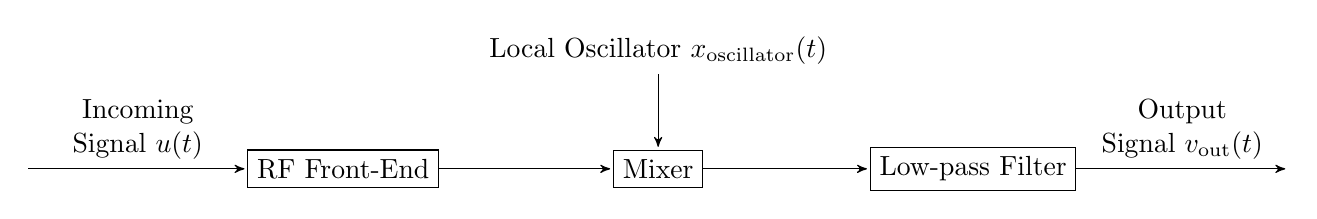
\begin{tikzpicture}[>=stealth',shorten >=1pt,auto,node distance=4cm,
                    block/.style={rectangle, draw, align=center}]
  % Nodes
  \node[block] (rf) {RF Front-End};
  \node[block, right of=rf] (mixer) {Mixer};
  \node[block, right of=mixer] (lpf) {Low-pass Filter};
  \node[coordinate, left of=rf] (input) {};
  \node[coordinate, right of=lpf] (output) {};

  % Edges
  \draw[->] (input) -- node[name=u, align=center] {Incoming\\Signal \(u(t)\)} (rf);
  \draw[->] (rf) -- node[name=v, align=center] {} (mixer);
  \draw[->] (mixer) -- node[name=w, align=center] {} (lpf);
  \draw[->] (lpf) -- node[name=x, align=center] {Output\\Signal \(v_{\text{out}}(t)\)} (output);

  % Labels
  \node[above of=mixer, node distance=1.5cm] (lo) {Local Oscillator \(x_{\text{oscillator}}(t)\)};
  \draw[->] (lo) -- (mixer);
\end{tikzpicture}



\subsection*{b) Power at Output of the Filter}
After mixing the DSB-SC AM signal \( u(t) \) with \( x_{\text{oscillator}}(t) \), we get:

\[
v(t) = u(t) \times x_{\text{oscillator}}(t) = A m(t) \cos(2\pi f_c t) \cos(2\pi f_c t + \theta)
\]
Expanding this, we get:
\[
v(t) = \frac{A}{2} m(t) \left[ \cos(2\theta) + \cos(4\pi f_c t + \theta) \right]
\]
The low-pass filter will remove the high-frequency component, leaving:
\[
v_{\text{out}}(t) = \frac{A}{2} m(t) \cos(2\theta)
\]
The power at the output of the filter will thus be:
\[
P_{\text{out}} = \frac{A^2}{4} P_m \cos^2(2\theta)
\]

\subsection*{c) Power for Different Angles}
We can calculate \( P_{\text{out}} \) for different values of \( \theta \) as:
\[
\begin{aligned}
    P_{\text{out}}(0^\circ) &= \frac{A^2}{4} P_m \\
    P_{\text{out}}(45^\circ) &= \frac{A^2}{8} P_m \\
    P_{\text{out}}(90^\circ) &= 0 \\
    P_{\text{out}}(135^\circ) &= \frac{A^2}{8} P_m
\end{aligned}
\]
These calculations show that the output power varies with the phase angle \( \theta \) of the local oscillator.


\newpage
\section*{Problem \#5}

The SNR in dB is defined as follows:
\[
\text{SNR}_{\text{dB}} = 10 \log_{10} \left( \frac{P}{\sigma_n^2} \right)
\]
where \(P\) is the signal power and \(\sigma_n^2\) is the noise power.

\subsubsection*{a) Factor of \( \sqrt{2} \) Increase in Amplitude}

When the amplitude increases by \( \sqrt{2} \), the signal power \(P\) changes as follows:
\[
P_{\text{new}} = 2 \times P_{\text{old}}
\]
The resulting SNR in dB becomes:
\[
\text{SNR}_{\text{dB, new}} = 10 \log_{10} (2) + \text{SNR}_{\text{dB, old}} \approx \text{SNR}_{\text{dB, old}} + 3 \text{ dB}
\]

\subsubsection*{b) Factor of 2 Increase in Amplitude}

When the amplitude increases by 2, the signal power \(P\) changes as follows:
\[
P_{\text{new}} = 4 \times P_{\text{old}}
\]
The resulting SNR in dB becomes:
\[
\text{SNR}_{\text{dB, new}} = 10 \log_{10} (4) + \text{SNR}_{\text{dB, old}} \approx \text{SNR}_{\text{dB, old}} + 6 \text{ dB}
\]

\subsubsection*{c) Factor of \( \sqrt{2} \) Decrease in Amplitude}

When the amplitude decreases by \( \sqrt{2} \), the signal power \(P\) changes as follows:
\[
P_{\text{new}} = \frac{P_{\text{old}}}{2}
\]
The resulting SNR in dB becomes:
\[
\text{SNR}_{\text{dB, new}} = \text{SNR}_{\text{dB, old}} - 10 \log_{10} (2) \approx \text{SNR}_{\text{dB, old}} - 3 \text{ dB}
\]

\subsubsection*{d) Factor of 2 Decrease in Amplitude}

When the amplitude decreases by 2, the signal power \(P\) changes as follows:
\[
P_{\text{new}} = \frac{P_{\text{old}}}{4}
\]
The resulting SNR in dB becomes:
\[
\text{SNR}_{\text{dB, new}} = \text{SNR}_{\text{dB, old}} - 10 \log_{10} (4) \approx \text{SNR}_{\text{dB, old}} - 6 \text{ dB}
\]

\newpage
\section*{Problem \#6}

The Signal-to-Noise Ratio (SNR) is given as 15 dB when the phase offset error \(\theta = 0^\circ\). We are asked to find the SNR in dB when the DSB-SC (Double Sideband-Suppressed Carrier) signal is demodulated with a phase error of \(\theta = 85^\circ\).

\subsection*{Solution}

The effect of the phase error \(\theta\) on SNR can be represented as a multiplication factor, which is \(\cos(\theta)\) for DSB-SC modulation. The original SNR is given in dB as 15 dB. The SNR in linear form can be calculated as:

\[
\text{SNR}_{\text{lin, old}} = 10^{\frac{\text{SNR}_{\text{dB, old}}}{10}} = 10^{\frac{15}{10}} = 31.62
\]
When a phase error of \(\theta = 85^\circ\) is introduced, the multiplication factor becomes \(\cos(85^\circ)\), which is approximately 0.0872. Therefore, the new SNR in linear form is:

\[
\text{SNR}_{\text{lin, new}} = 31.62 \times \cos(85^\circ) \approx 31.62 \times 0.0872 \approx 2.757
\]
Finally, to convert this back to dB, we use:

\[
\text{SNR}_{\text{dB, new}} = 10 \log_{10}(\text{SNR}_{\text{lin, new}}) = 10 \log_{10}(2.757) \approx 4.4 \text{ dB}
\]
So, the SNR drops to approximately 4.4 dB when the phase error is \(\theta = 85^\circ\).

\newpage
\section*{Problem \#7}

We are given that \(N\) message signals need to be transmitted in different frequency bands in a non-overlapping manner. The maximum baseband bandwidth of any of the signals is \(44 \, \text{kHz}\). We aim to find the total spectrum required for the entire multiplexed signal under three modulation schemes: conventional AM, DSB-SC AM, and SSB-AM.

\subsection*{Solution}

\subsubsection*{a) Conventional AM}

In conventional Amplitude Modulation (AM), each message signal requires a bandwidth of twice its maximum baseband bandwidth for the sidebands. Therefore, the bandwidth for one channel in conventional AM is \(2 \times 44 \, \text{kHz} = 88 \, \text{kHz}\).

For \(N = 16\) such non-overlapping channels, the total bandwidth required would be:

\[
\text{Total Bandwidth}_{\text{Conventional AM}} = 16 \times 88 \, \text{kHz} = 1408 \, \text{kHz}
\]

\subsubsection*{b) DSB-SC AM}

In Double Sideband-Suppressed Carrier (DSB-SC) AM, similar to conventional AM, each channel would also require \(2 \times 44 \, \text{kHz} = 88 \, \text{kHz}\).

So, for \(N = 16\), the total bandwidth would be:

\[
\text{Total Bandwidth}_{\text{DSB-SC AM}} = 16 \times 88 \, \text{kHz} = 1408 \, \text{kHz}
\]

\subsubsection*{c) SSB-AM}

In Single Sideband (SSB) AM, only one sideband is transmitted. Therefore, the bandwidth for one channel in SSB-AM is \(44 \, \text{kHz}\).

For \(N = 16\), the total bandwidth required would be:

\[
\text{Total Bandwidth}_{\text{SSB-AM}} = 16 \times 44 \, \text{kHz} = 704 \, \text{kHz}
\]

In summary, the total spectrum requirements for the entire multiplexed signal are 1408 kHz for both Conventional AM and DSB-SC AM, and 704 kHz for SSB-AM.

\newpage
\section*{Problem \#8}

\textbf{Problem Statement:} Assume that the message signal \( m(t) = 3\cos(2\pi 100t) + \sin(2\pi 300t) \). We transmit the signal with conventional AM, where the carrier is \( c(t) = \cos(2\pi 105t) \) and the modulation index is 0.85.

\subsection*{Solutions}

\subsubsection*{a) Maximum of \( |m(t)| \)}

To find the maximum of \( |m(t)| \), we can use derivatives to locate the extrema points.

The given message signal is:
\[
m(t) = 3\cos(2\pi 100t) + \sin(2\pi 300t)
\]

Taking the derivative, \( m'(t) \), and setting it to zero gives us the critical points:
\[
m'(t) = -3 \times 2\pi 100 \sin(2\pi 100t) + 2\pi 300 \cos(2\pi 300t) = 0
\]

We have \( m'(t) = -3 \times 2\pi 100 \sin(2\pi 100t) + 2\pi 300 \cos(2\pi 300t) \), and we set it equal to zero to find the critical points.

\[
0 = -3 \times 2\pi 100 \sin(2\pi 100t) + 2\pi 300 \cos(2\pi 300t)
\]

Simplifying the equation, we get:
\[
\sin(2\pi 100t) = \cos(2\pi 300t)
\]

As \( \sin(\theta) = \cos(\frac{\pi}{2} - \theta) \), we have:

\[
2\pi 300t = \frac{\pi}{2} - 2\pi 100t
\]

Solving for \( t \):
\[
t = \frac{1}{1600}
\]
Since the function \( m(t) \) is periodic and we are interested in the maximum value, let's consider a positive value of \( t \) which would be \( t = \frac{1}{1600} \).
\newline \newline
Now we plug this back into the original function \( m(t) \):

\[
m\left(\frac{1}{1600}\right) = 3\cos\left(2\pi 100 \times \frac{1}{1600}\right) + \sin\left(2\pi 300 \times \frac{1}{1600}\right)
\]

\[
m\left(\frac{1}{1600}\right) = 3\cos\left(\frac{\pi}{8}\right) + \sin\left(\frac{3\pi}{8}\right)
\]

\[
m\left(\frac{1}{1600}\right) = 3.6955181300
\]
Since \( |m(t)| \) is what we are interested in, the maximum \( |m(t)| \) is approximately 3.70 when \( t = \frac{1}{1600} \).
\newline \newline
Thus, the maximum of \( |m(t)| \) is approximately 3.70 when evaluated at \( t = \frac{1}{1600} \).


\subsubsection*{b) Normalized Message}

The normalized message signal \( m_{\text{norm}}(t) \) is obtained by dividing the message signal \( m(t) \) by its maximum value \( |m(t)|_{\text{max}} \), which is approximately 3.70 at \( t = \frac{1}{1600} \):
\[
m_{\text{norm}}(t) = \frac{3\cos(2\pi 100t) + \sin(2\pi 300t)}{3.70}
\]
This normalized message signal \( m_{\text{norm}}(t) \) reflects the original \( m(t) \) divided by the maximum value 3.70.
\subsubsection*{c) Power of Normalized Message}

To find the power of the normalized message \( P_{\text{norm}} \), we first distribute the constant factor of \( \frac{1}{3.7} \) to both trigonometric terms:
\[
P_{\text{norm}} = \frac{1}{T} \int_0^T \left| 0.8108\cos(2\pi 100t) + 0.2703\sin(2\pi 300t) \right|^2 \, dt
\]

\subsubsection*{Simplified Power of Individual Terms Using Standard Power Formula}

For a standard sinusoidal waveform, the power is calculated as \( \frac{A^2}{2} \).

1. For \( 0.8108\cos(2\pi 100t) \), the power is \( \frac{(0.8108)^2}{2} = \frac{0.6574}{2} = 0.3287 \).

2. For \( 0.2703\sin(2\pi 300t) \), the power is \( \frac{(0.2703)^2}{2} = \frac{0.0731}{2} = 0.0366 \).

\subsubsection*{Final Power of Normalized Message}

The total power \( P_{\text{norm}} \) would be a sum of these individual powers. Therefore, for \( T = \frac{1}{100} \), \( P_{\text{norm}} = 0.3287 + 0.0366 = 0.3653 \).

\subsubsection*{d) Calculate the Power in the Carrier Component and Information Component of the Conventional AM Signal}

To calculate the power in the carrier and information components, we will use the following formulas.

\begin{equation}
P_c = \frac{A^2}{2}
\end{equation}
where \( A = 1 \) is the amplitude of the carrier signal \( c(t) \).
\newline \newline
The power in the information component \( P_{\text{info}} \) can be calculated using the Modulation Index \( \mu = 0.85 \) as:
\begin{equation}
P_{\text{info}} = (|m(t)|_{\text{max}} \times \text{Modulation Index})^2 = \frac{1}{2} \times (0.85)^2 \times 0.3653 
\end{equation}
By calculating, \( P_{\text{info}} = 0.1319 \).
Finally, the total power \( P_{\text{total}} \) of the AM signal will be the sum of the carrier and information component powers:
\begin{equation}
P_{\text{total}} = P_c + P_{\text{info}} = \frac{1}{2} + 0.1319 = 0.6319
\end{equation}

\end{document}
